\section{仿真实验}\label{sec:experiments}
\subsection{场景、比较方法与评价设置}\label{sec:baselines}
四站坐标分别为$(500,0)$、$(0,500)$、$(-500,0)$和$(0,-500)$\,m。以最大站间距离定义基线$R=\max_{l,v}\|\bm r_l-\bm r_v\|_2=1000$\,m。搜索区域为$[-1000,1000]^2$\,m$^2$，真实源位置为连续坐标，不要求落在初始网格上。两源采用独立BPSK符号，经根升余弦（RRC）脉冲成形；符号率$R_s=10$\,MHz、滚降系数$\alpha_{\mathrm{RRC}}=0.25$，对应名义带宽$B=(1+\alpha_{\mathrm{RRC}})R_s=12.5$\,MHz。表\ref{tab:scenario}汇总公共设置。

\begin{table}[htbp]\centering\small
\caption{公共仿真参数。}\label{tab:scenario}
\begin{tabularx}{.96\linewidth}{@{}lX@{}}\toprule
参数 & 设置\\\midrule
接收站／源数 & 四个同步单天线站；已知$K=2$\\
传播 & 自由空间相对幅度$1/d$与基带时延；$c_0=299792458$\,m/s\\
波形 & 独立BPSK；RRC成形，符号率10\,MHz，滚降0.25\\
中心与名义带宽 & 两源中心均为0；带宽均为12.5\,MHz\\
采样与记录 & 50\,MHz；8192点；163.84\,$\mu$s\\
处理频带 & $[-7,7]$\,MHz；完整记录DFT保留2293个频点\\
噪声与信噪比 & 时域复噪声方差1；源B四站平均带内SNR为6\,dB\\
平均接收功率差 & 0、3、6、9、12、15\,dB；固定源B与噪声，仅缩放源A\\
初始网格 & 各方法统一20\,m，$101\times101=10201$点\\
候选间距 & 30\,m；AP联合版本分别保留1、2、5个候选\\
正式规模 & 20布局$\times$20随机实现$\times$6档功率差，共2400条\\
共同子集 & 各布局预先固定2次实现，保留全部功率差，共240条\\\bottomrule
\end{tabularx}
\end{table}

两源的符号、波形初相和定时独立。同一布局与随机实现的六档功率差共用波形和噪声，因而可以直接观察另一源增强带来的变化。源A为功率扫描源，源B为固定源；在正功率差下分别称强源和弱源，0\,dB时采用A／B标记。各方法只处理预先指定的公共频带$[-7,7]$\,MHz，在名义带宽两侧各留0.75\,MHz保护带，不提供逐源波形或频谱。筛选频点不重新缩放DFT，也不作逐站混合功率归一化。

正式比较采用20个布局，覆盖双源均在站内、A外B内、A内B外和双源均在站外四类构型，每类5个。站内指四站凸包内部，站外仍位于搜索区域内。几何生成排除距任一站小于150\,m、距中心小于100\,m、距站点对连线小于50\,m的位置，两源间距至少300\,m。位置按预定几何约束生成，不按定位结果筛选。图\ref{fig:formalgeometry}展示全部布局。核心方法使用全部2400条观测；八类方法使用其中预先固定的共同240条，不将子集与主批重复计数。
\begin{figure}[htbp]\centering
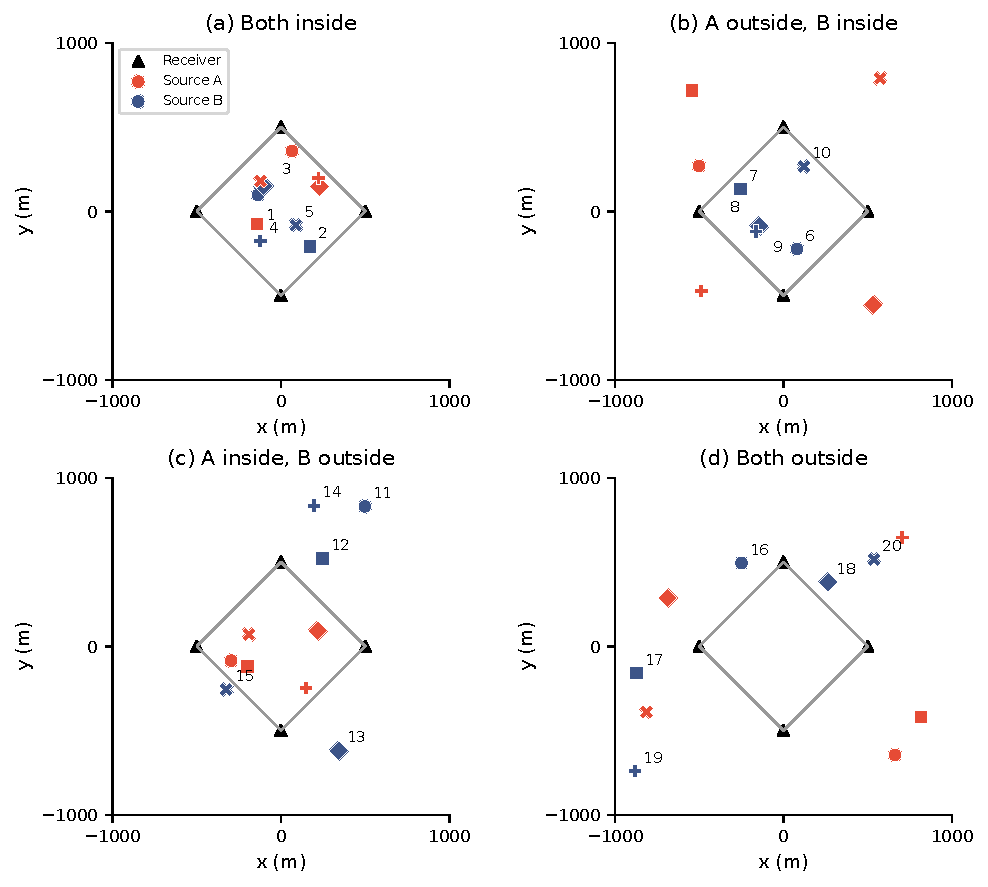
\includegraphics[width=.88\linewidth]{figures/formal_geometry.pdf}
\caption{20个源站布局，每类5个。黑色三角形为接收站，灰色菱形边界为站点凸包；同一面板内，相同形状的两个标记为一对源，红色为源A、蓝色为源B，数字为布局编号。0\,dB时两源平均接收功率相同。}\label{fig:formalgeometry}
\end{figure}

所有方法共享IQ观测、已知传播信息、搜索区域和20\,m初始网格，保留各自的连续精修。LS谱、MUSIC、MVDR、AP、块NOMP、SBL、多初值联合ML和GA联合ML的本场景准则列于附录\ref{app:baselines}；具体参数见表\ref{tab:parameters}。多初值ML采用去重的谱峰组合与Sobol空间覆盖起点，GA采用128个体，避免因重复初始化削弱搜索覆盖。MUSIC以同一记录的四个片段估计协方差，按扣除噪声后的观测功率加权；MVDR-known使用八个片段，相对对角加载为0.01。两者均只分析公共处理带内的频点，不将MVDR-known称为原版DPD-HR。
\par\begin{table}[htbp]\centering\footnotesize
\caption{正式比较采用的方法参数。连续位置优化不受20\,m网格量化。}\label{tab:parameters}
\begin{tabularx}{\linewidth}{@{}p{.18\linewidth}p{.27\linewidth}X@{}}\toprule
版本 & 核心操作 & 参数\\\midrule
LS谱 & 单源LS谱取两个峰 & 共同20 m网格；同谱连续精修\\
MUSIC & 噪声子空间宽带汇聚 & 4段；超噪声功率加权；已知K\\
MVDR-known & 加载协方差逆谱 & 8段；相对加载0.01\\
充分AP & 反复全域条件更新 & 候选5；循环上限6；正常连续精修\\
交替／联合AP & 相同分支，改变精修方式 & 候选1/2/5；每次局部上限100；共同投影梯度阈值$10^{-8}$\\
VP-BNOMP & 残差发现、消元Newton、共同LS & 循环上限200；每次Newton最多5步；步长上限50 m\\
固定系数BNOMP & 原文对应的固定系数更新 & 循环上限10000；能量阈值$10^{-8}$；局部小步阈值0.01 m\\
多初值联合ML & 同一联合LS目标 & 8个唯一初值：4谱峰+4 Sobol；L-BFGS-B\\
GA联合ML & 同一联合LS目标 & 种群128；最多200代；连续30代停滞停止\\
宽带SBL & 共享功率、离网字典、单点$\gamma$ & 最多300轮；每5轮离网更新；8个活动点；原生停止\\
\bottomrule\end{tabularx}\end{table}
\par
运行环境为Windows、Python 3.10.20、NumPy 2.2.6和PyTorch 2.8.0+cu129，GPU为NVIDIA GeForce RTX 4070 Ti SUPER，CPU计算线程设为20。响应与目标使用双精度实数／复数运算。
\par

\FloatBarrier
\paragraph{定位评价}
设真实与估计集合分别为$X=\{\bm p_k\}$、$Y=\{\widehat{\bm p}_j\}$。容许误差预先设为基线的2\%，即$r=0.02R=20$\,m，与初始网格步长分别定义。成功评价在距离不超过$r$的关联中先最大化一对一匹配数，再最小化平方距离和；双源成功要求两源同时匹配，单个估计不能重复对应两个真源。位置误差则使用最小平方距离指派\cite{Kuhn1955}：
\begin{equation}
 \pi^*=\arg\min_{\pi}\sum_{k=1}^{K}\|\bm p_k-\widehat{\bm p}_{\pi(k)}\|_2^2,
 \qquad e_{ik}=\|\bm p_{ik}-\widehat{\bm p}_{i,\pi^*(k)}\|_2 .\label{eq:assignment}
\end{equation}
其中$i$为观测编号，$k$为源编号，$\pi$为估计编号的排列，$e_{ik}$单位为m。对$n$条观测，RMSE和经验累计分布函数（CDF）为
\begin{equation}
 \operatorname{RMSE}_k=\sqrt{\frac1n\sum_{i=1}^{n}e_{ik}^2},\qquad
 \widehat F_k(t)=\frac1n\sum_{i=1}^{n}\mathbf 1(e_{ik}\le t).\label{eq:rmseCDF}
\end{equation}
式中$\mathbf 1$为示性函数，P95为误差的第95百分位数。RMSE和CDF使用全部样本，包括未达到成功门槛的样本。GOSPA\cite{Rahmathullah2017}保留为辅助集合指标，取$p=2$、$c=100$\,m、$\alpha=2$，其定义为
\begin{equation}
 d_{\mathrm G}(X,Y)^2=\min_{\gamma}\left[
 \sum_{(k,j)\in\gamma}\|\bm p_k-\widehat{\bm p}_j\|^2
 +\frac{c^2}{2}\left(|X|+|Y|-2|\gamma|\right)\right].\label{eq:gospa}
\end{equation}
这里$\gamma$为一对一部分关联，$|\cdot|$表示集合基数。正文以成功率、RMSE、CDF和耗时为主要比较依据。

\paragraph{成本与统计}
完整算法时间包含IQ输入后的DFT、频带筛选、传输、搜索、系数重估和精修，GPU计时同步，公共预热单列。在线轨迹记录计入登记墙钟，磁盘持久化及事后精度证书不计入求解时间；各方法独立承担搜索与初始化成本。目标、梯度、响应及循环调用分别统计，包含梯度计算的目标请求不与梯度次数相加。布局内同一实现的六档功率差保持配对；不确定性按构型类别、布局及随机实现分层重采样。核心比较和共同子集比较分别统计。

\subsection{核心方法的总体定位表现}\label{sec:coreformal}
多候选的主要收益是恢复单一起点遗漏的弱源。表\ref{tab:formalcore}给出全部2400条观测的结果：五候选MCJ-AP成功2376条，将单候选的95\%成功率提高至99\%，平均耗时为0.718\,s。两者的强源RMSE均约0.897\,m，说明弱源恢复没有以降低强源精度为代价。VP-BNOMP及其末端联合版本均成功2278条，追加末端精修没有增加本批成功数。
\begin{table}[htbp]\centering\small
\caption{全部2400条观测的核心比较。成功门槛20\,m；RMSE和P95单位为m，时间单位为s。}\label{tab:formalcore}
\begin{tabular}{@{}lrrrrrr@{}}\toprule
方法 & 双源成功 & 成功率/\% & 强源RMSE & 弱源RMSE & 弱源P95 & 时间\\\midrule
单候选交替AP & 2280/2400 & 95.00 & 0.897 & 107.258 & 25.194 & 0.4390\\
单候选联合AP & 2280/2400 & 95.00 & 0.897 & 107.265 & 25.194 & 0.3958\\
双候选联合AP & 2280/2400 & 95.00 & 0.897 & 103.698 & 25.194 & 0.4704\\
五候选联合AP & 2376/2400 & 99.00 & 0.896 & 46.984 & 3.845 & 0.7180\\
VP-BNOMP & 2278/2400 & 94.92 & 0.893 & 73.374 & 222.325 & 0.8162\\
VP-BNOMP＋联合 & 2278/2400 & 94.92 & 0.897 & 76.261 & 215.181 & 0.8474\\
\bottomrule\end{tabular}\end{table}

\begin{figure}[htbp]\centering
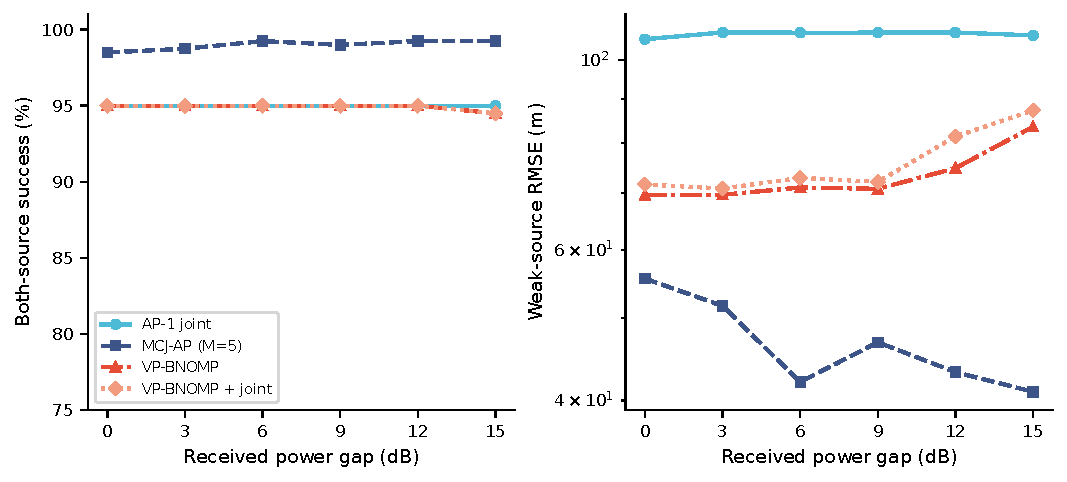
\includegraphics[width=\linewidth]{figures/formal_core.pdf}
\caption{核心比较的双源成功率与弱源RMSE。每档功率差400条，合计2400条；同一实现的功率扫描保持配对。RMSE计入全部失败，曲线波动主要受困难布局中的少量大误差影响。}\label{fig:formalcore}
\end{figure}

图\ref{fig:formallayouts}进一步显示收益来自何处。单候选在布局4的120条观测上全部失败，五候选恢复其中96条；其余布局原已成功，增加候选没有造成成功转失败。保留多个起点的作用集中在困难构型，而不是对所有观测一律提高精度。
\begin{figure}[htbp]\centering
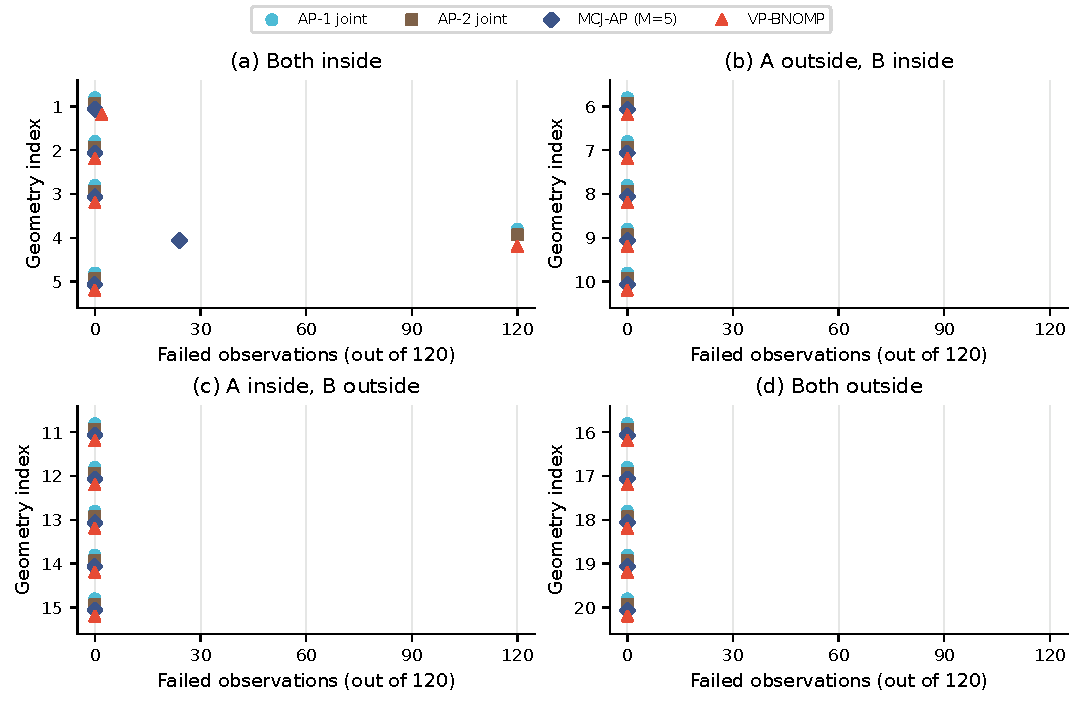
\includegraphics[width=\linewidth]{figures/formal_layouts.pdf}
\caption{各布局的双源失败数，每布局120条。四个面板对应四类构型，零表示该布局全部成功；不同标记在纵向稍作错开，便于辨认重合结果。}\label{fig:formallayouts}
\end{figure}

五候选弱源P95为3.85\,m，RMSE为46.98\,m：大多数观测已有米级精度，少量远距离误差则拉高了RMSE。图\ref{fig:formalcore}中的非单调折线也来自这一统计特点。六档功率差下，每档400条中有3--6条失败，均来自布局4，并贡献各档超过99.7\%的弱源平方误差。仅作为归因检查，其余19个布局的弱源RMSE随功率差从1.31\,m增至1.93\,m。因此，整体RMSE的折线不能直接解释成强源增强有利于定位；它主要反映少量候选选择失败的数量与距离变化。正文主结果仍包含全部布局和失败，图\ref{fig:formalcdfcost}同时展示完整误差分布。

\FloatBarrier
\subsection{八类方法的共同观测比较}\label{sec:commonformal}
在相同观测上，MCJ-AP以更低成本达到了充分AP和SBL的恢复水平。表\ref{tab:formalcommon}使用各布局两次固定实现及全部六档功率差，共240条。五候选联合AP、充分AP和宽带SBL均全部成功，平均完整耗时分别为0.708\,s、8.908\,s和44.130\,s。固定系数BNOMP与当前VP-BNOMP均成功228条，后者平均耗时由2.942\,s降至0.836\,s。两种NOMP的整算法比较还包含系数重估时序、接受规则和导数实现差别；第\ref{sec:mechanismresults}节另讨论局部消元机制。
\begin{table}[htbp]\centering\small
\caption{同一240条观测上的基线与提出方法比较。成功门槛20\,m；RMSE和P95单位为m，时间单位为s。}\label{tab:formalcommon}
\begin{tabular}{@{}lrrrrrr@{}}\toprule
方法 & 双源成功 & 成功率/\% & 强源RMSE & 弱源RMSE & 弱源P95 & 时间\\\midrule
LS谱取峰 & 38/240 & 15.83 & 191.982 & 845.184 & 1708.755 & 0.2368\\
宽带MUSIC & 151/240 & 62.92 & 93.515 & 646.892 & 1701.876 & 0.2015\\
MVDR-known & 75/240 & 31.25 & 320.684 & 804.082 & 1706.625 & 0.1925\\
充分AP & 240/240 & 100.00 & 0.876 & 1.596 & 4.229 & 8.9076\\
固定系数BNOMP & 228/240 & 95.00 & 0.906 & 89.706 & 30.998 & 2.9416\\
VP-BNOMP & 228/240 & 95.00 & 0.875 & 84.723 & 18.993 & 0.8359\\
多初值联合ML & 45/240 & 18.75 & 256.061 & 776.935 & 1719.566 & 1.2227\\
GA联合ML & 185/240 & 77.08 & 279.056 & 501.231 & 1634.174 & 8.0702\\
宽带SBL & 240/240 & 100.00 & 1.096 & 3.743 & 8.962 & 44.1296\\
五候选联合AP & 240/240 & 100.00 & 0.876 & 1.596 & 4.229 & 0.7081\\
\bottomrule\end{tabular}\end{table}

\begin{figure}[htbp]\centering
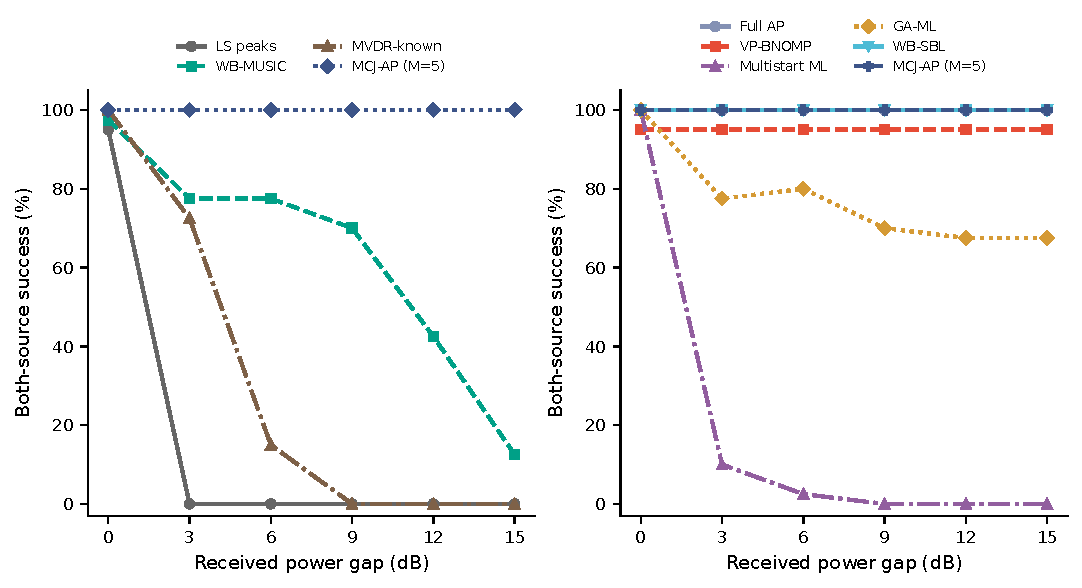
\includegraphics[width=\linewidth]{figures/formal_common.pdf}
\caption{共同240条观测的功率差扫描，每档40条。左侧比较谱方法，右侧比较逐源与联合求解方法；两个面板使用同一五候选AP参照。}\label{fig:formalcommon}
\end{figure}

\begin{samepage}
图\ref{fig:formalcommon}显示，MUSIC与MVDR-known在功率差增大后明显退化，整体成功率分别为62.92\%和31.25\%；LS谱取峰为15.83\%。逐源或联合拟合能够更好地处理本组混合观测。多初值ML成功率为18.75\%，充分AP则达到100\%；二者使用同一联合目标，结果差别体现了初始化与搜索路径的重要性。GA成功率为77.08\%，平均耗时为8.070\,s。
\end{samepage}

上述八类比较均使用共同240条，核心方法表则使用全部2400条。SBL有226条按原生稳定条件停止、14条达到300轮上限；VP-BNOMP在主批有86条达到200轮上限，均按最终输出统计。辅助GOSPA、耗时P95与共同子集停止状态见表\ref{tab:auxiliary}。
\begin{figure}[htbp]\centering
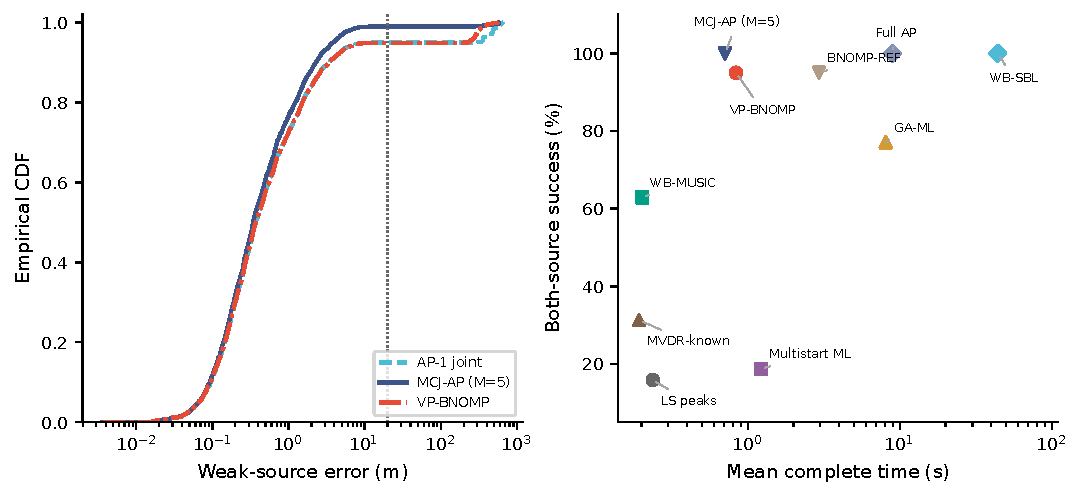
\includegraphics[width=\linewidth]{figures/formal_cdf_cost.pdf}
\caption{误差分布与可靠性--成本取舍。左：全部2400条核心观测的弱源CDF，虚线标出20\,m；右：同一240条共同子集的双源成功率与平均完整耗时。两个面板的样本范围分别标明，不跨样本范围排名。}\label{fig:formalcdfcost}
\end{figure}

\FloatBarrier
\subsection{候选保留提高可靠性，联合精修减少计算}\label{sec:apresults}
两项改动承担不同作用。表\ref{tab:apablation}中，候选数为1和2的联合AP均成功2280条，五候选增至2376条。增加到第二候选尚未覆盖本批困难区域，保留更多有效起点才带来恢复。图\ref{fig:formalablation}将候选数量的收益与相同五候选下的精修成本分别展示。
\begin{table}[htbp]\centering\small
\caption{AP候选数与精修方式的消融，全部2400条观测。}\label{tab:apablation}
\begin{tabular}{@{}lrrrr@{}}\toprule
配置 & 双源成功 & 时间/s & 联合目标计算 & 梯度计算\\\midrule
单候选交替AP & 2280 & 0.4390 & 39.76 & 37.76\\
单候选联合AP & 2280 & 0.3958 & 28.69 & 26.69\\
双候选联合AP & 2280 & 0.4704 & 49.63 & 46.63\\
五候选联合AP & 2376 & 0.7180 & 120.36 & 114.36\\
\bottomrule\end{tabular}\end{table}

\begin{figure}[htbp]\centering
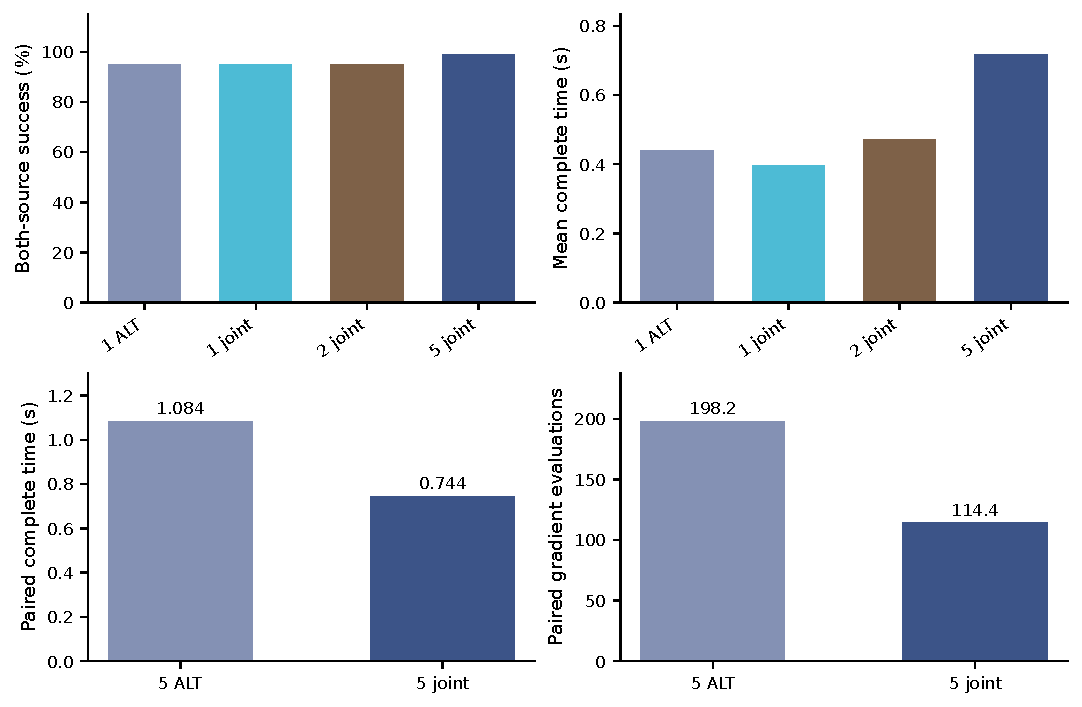
\includegraphics[width=\linewidth]{figures/formal_ablation.pdf}
\caption{AP的两项作用。上行：原2400条主批中的候选数与精修消融；下行：同一2400条输入上，五候选交替／联合完整配对的耗时及梯度计算。ALT为交替精修，joint为联合精修。上下两批分别计时，不跨批计算加速比。}\label{fig:formalablation}
\end{figure}

单候选配对先说明了联合精修的省时作用：相同成功数和接近的RMSE下，平均耗时从0.439\,s降至0.396\,s，减少9.84\%。平均耗时差（联合减交替）的95\%分层配对区间为$[-0.0496,-0.0367]$\,s；目标计算从39.76次降至28.69次，梯度计算从37.76次降至26.69次。

表\ref{tab:fivepair}给出主方法的直接配对验证。两种版本对每条观测使用完全相同的五个初始候选，在同一完整目标和投影梯度阈值下停止；运行顺序交错，共2400对、4800次求解。两者均成功2376条，成功／失败身份逐例一致，强弱源RMSE也几乎相同。联合精修将平均完整耗时从1.0840\,s降至0.7441\,s，减少31.36\%；耗时差的95\%分层配对区间为$[-0.3691,-0.3121]$\,s。
\begin{table}[htbp]\centering\small
\caption{相同五候选、共同停止精度下的完整配对，2400对。}\label{tab:fivepair}
\begin{tabular}{@{}lrrrrr@{}}\toprule
精修方式 & 双源成功 & 强源RMSE/m & 弱源RMSE/m & 时间/s & 梯度次数\\\midrule
交替 & 2376 & 0.896 & 46.983 & 1.0840 & 198.21\\
联合 & 2376 & 0.896 & 46.984 & 0.7441 & 114.36\\
\bottomrule\end{tabular}\end{table}


省时与计算量减少一致：平均联合目标计算从204.21次降至120.36次，梯度计算从198.21次降至114.36次，后者减少约42.30\%。两种版本选中分支均满足共同梯度条件，全部候选中有两次交替精修触及安全迭代上限，其结果仍计入统计。由此，多候选保留了困难弱源的有效起点，联合精修则以更少局部计算处理这些候选，两者共同构成MCJ-AP的可靠性与效率收益。

\FloatBarrier
\subsection{波形消元更新的机制与效率}\label{sec:mechanismresults}
式\eqref{eq:schur}给出了固定系数与消元曲率之间的关系。位置改变时，波形系数可以补偿一部分响应变化，固定系数曲率没有扣除这部分耦合，可能产生反复的小步。局部消元同时改变更新方向和试探位置的目标计算，因此应与保留相同外层时序的参照配对，区分局部更新收益与整套实现差别。

\pending{最终消元NOMP版本确定后，在此统一填写算法对应、固定系数／消元对照、收敛轨迹和完整成本；PROFILE相关正式结果及主批验证暂不填入。}

\subsection{时间轨迹与候选机制解释}\label{sec:timecases}
图\ref{fig:formaltime}展示好结果何时出现，而不只比较算法何时结束。在共同240条观测上，五候选联合AP在0.75\,s保存点达到全部成功，充分AP在2\,s达到相同成功数，SBL在30\,s达到相同成功数。尚无双源输出的观测按未成功计；RMSE仅在全部观测有输出后显示。曲线重放算法当时保留的解。
\begin{figure}[htbp]\centering
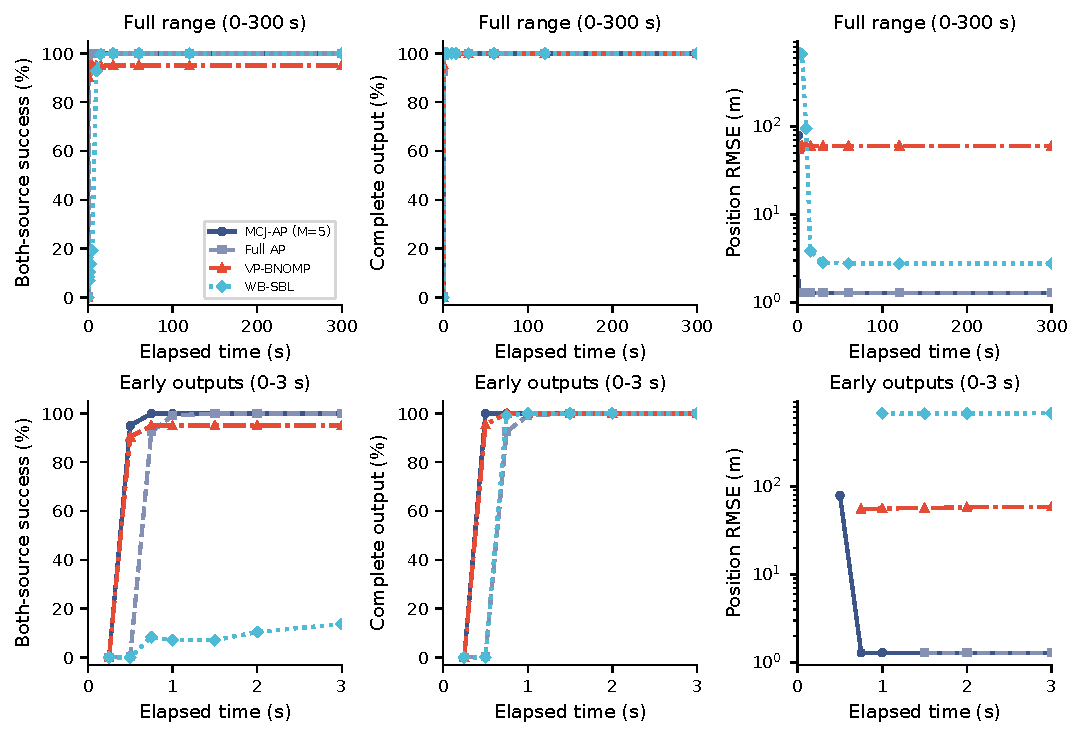
\includegraphics[width=\linewidth]{figures/formal_time.pdf}
\caption{共同240条观测的保存输出轨迹。横轴均为线性时间，上行显示0--300\,s全时段，下行放大0--3\,s；三列依次为双源成功率、完整输出比例和位置RMSE。正常停止后保持最终值，RMSE纵轴仍用对数刻度。连接线表示保存点之间的变化，不额外规定算法停止时刻。}\label{fig:formaltime}
\end{figure}

充分AP和SBL在最终停止前已取得高成功率，因此取得结果的时间与完成全部计算的时间需要分别观察。五候选AP更早恢复了全部共同样本；各方法的时间曲线与最终成本采用相同观测和计时口径。

图\ref{fig:formalcandidates}解释为什么需要保留多个条件候选。上行中，前四个候选都进入远端错误区域，第五候选则接近真实源B。联合精修后，第五分支得到更低残差，源B误差约0.09\,m。下行的五个候选均落在远端高分带，最近起点仍距源B约397\,m，局部精修未能恢复。两个案例说明，粗谱最高分与精修后的最佳位置并不等价；候选保留通过增加有效起点提高可靠性，其效果取决于候选是否覆盖正确区域。
\begin{figure}[htbp]\centering
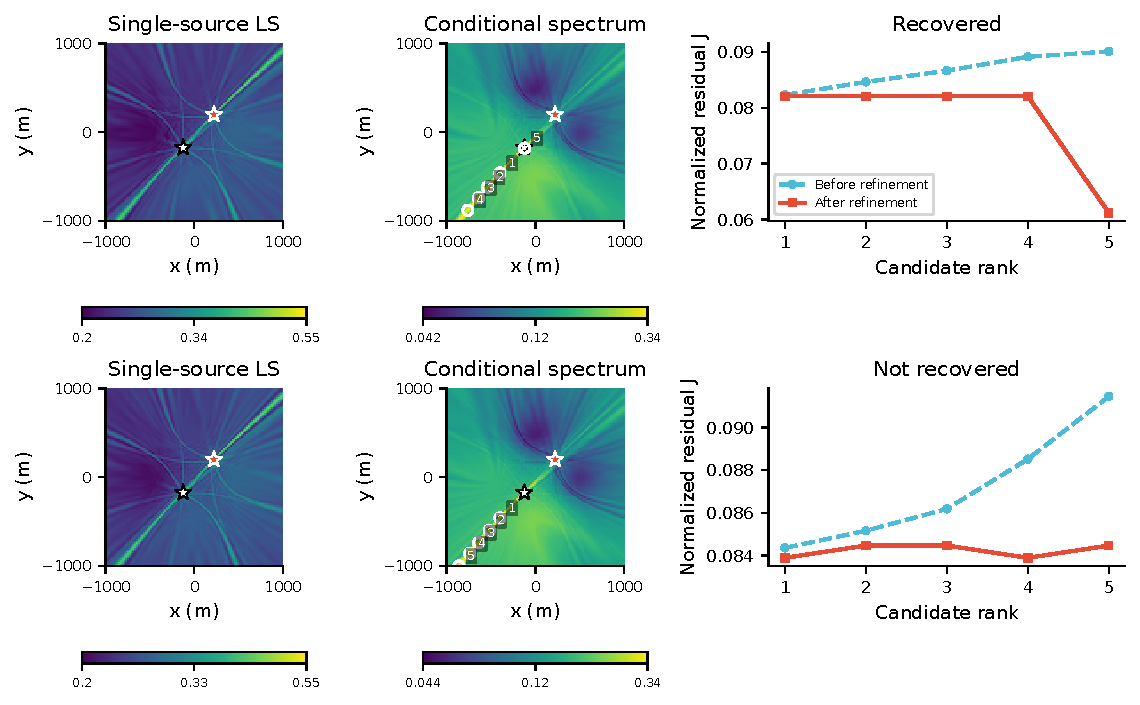
\includegraphics[width=\linewidth]{figures/formal_candidates.pdf}
\caption{同一困难构型的两个0\,dB事后机制案例。左列为单源LS谱，中列为条件谱，右列为候选精修前后残差；上行为恢复案例，下行为未恢复案例。红色和白色星号分别标示源A、源B，空心圆为条件候选。谱图采用对数色标，右列连接线仅连接候选编号，不表示实际迭代路径。}\label{fig:formalcandidates}
\end{figure}

第\ref{sec:complexity}节的复杂度分析与实际调用量相对应：单／五候选AP均只作两次全域网格扫描，增加分支主要增加连续目标和梯度计算；固定系数与消元NOMP则需比较局部导数调用和循环成本。这些计数用于解释候选覆盖与局部更新各自带来的开销和收益。
